% !TEX root = ../Thesis.tex

\newcommand{\microm}{\ensuremath{\mu m}}
\newcommand{\rphi}{$R$-$\phi$}

\chapter{The LHC and the ATLAS Detector} \label{sec:lhc_atlas_detector}

\section{The Large Hadron Collider} \label{sec:the_large_hadron_collider}

The Large Hadron Collider (LHC)~\cite{LHC} is a proton ring collider located at the European Centre for Nuclear Research (CERN). The main LHC ring is housed in the tunnel which previously contained the Large Electron-Positron collider. The LHC ring is 27km in circumference and located approximately 175m underground. The LHC services four different experiments located at four interaction points around the beam-pipe (Figure~\ref{fig:DetectorLHCLayout}). A toroidal LHC apparatus (ATLAS, the experiment used for this thesis), the compact muon solenoid (CMS), a large ion collider (ALICE) experiment and the LHC beauty (LHCb) experiment. 

ATLAS and CMS are general purpose detectors designed to support a varied physics programme, from SM physics like top quark measurements to BSM searches such as supersymmetry. ALICE and LHCb are more specialized experiments which focus on heavy ions and $b$ physics, respectively.

\begin{figure}[htbp]
  \centering
  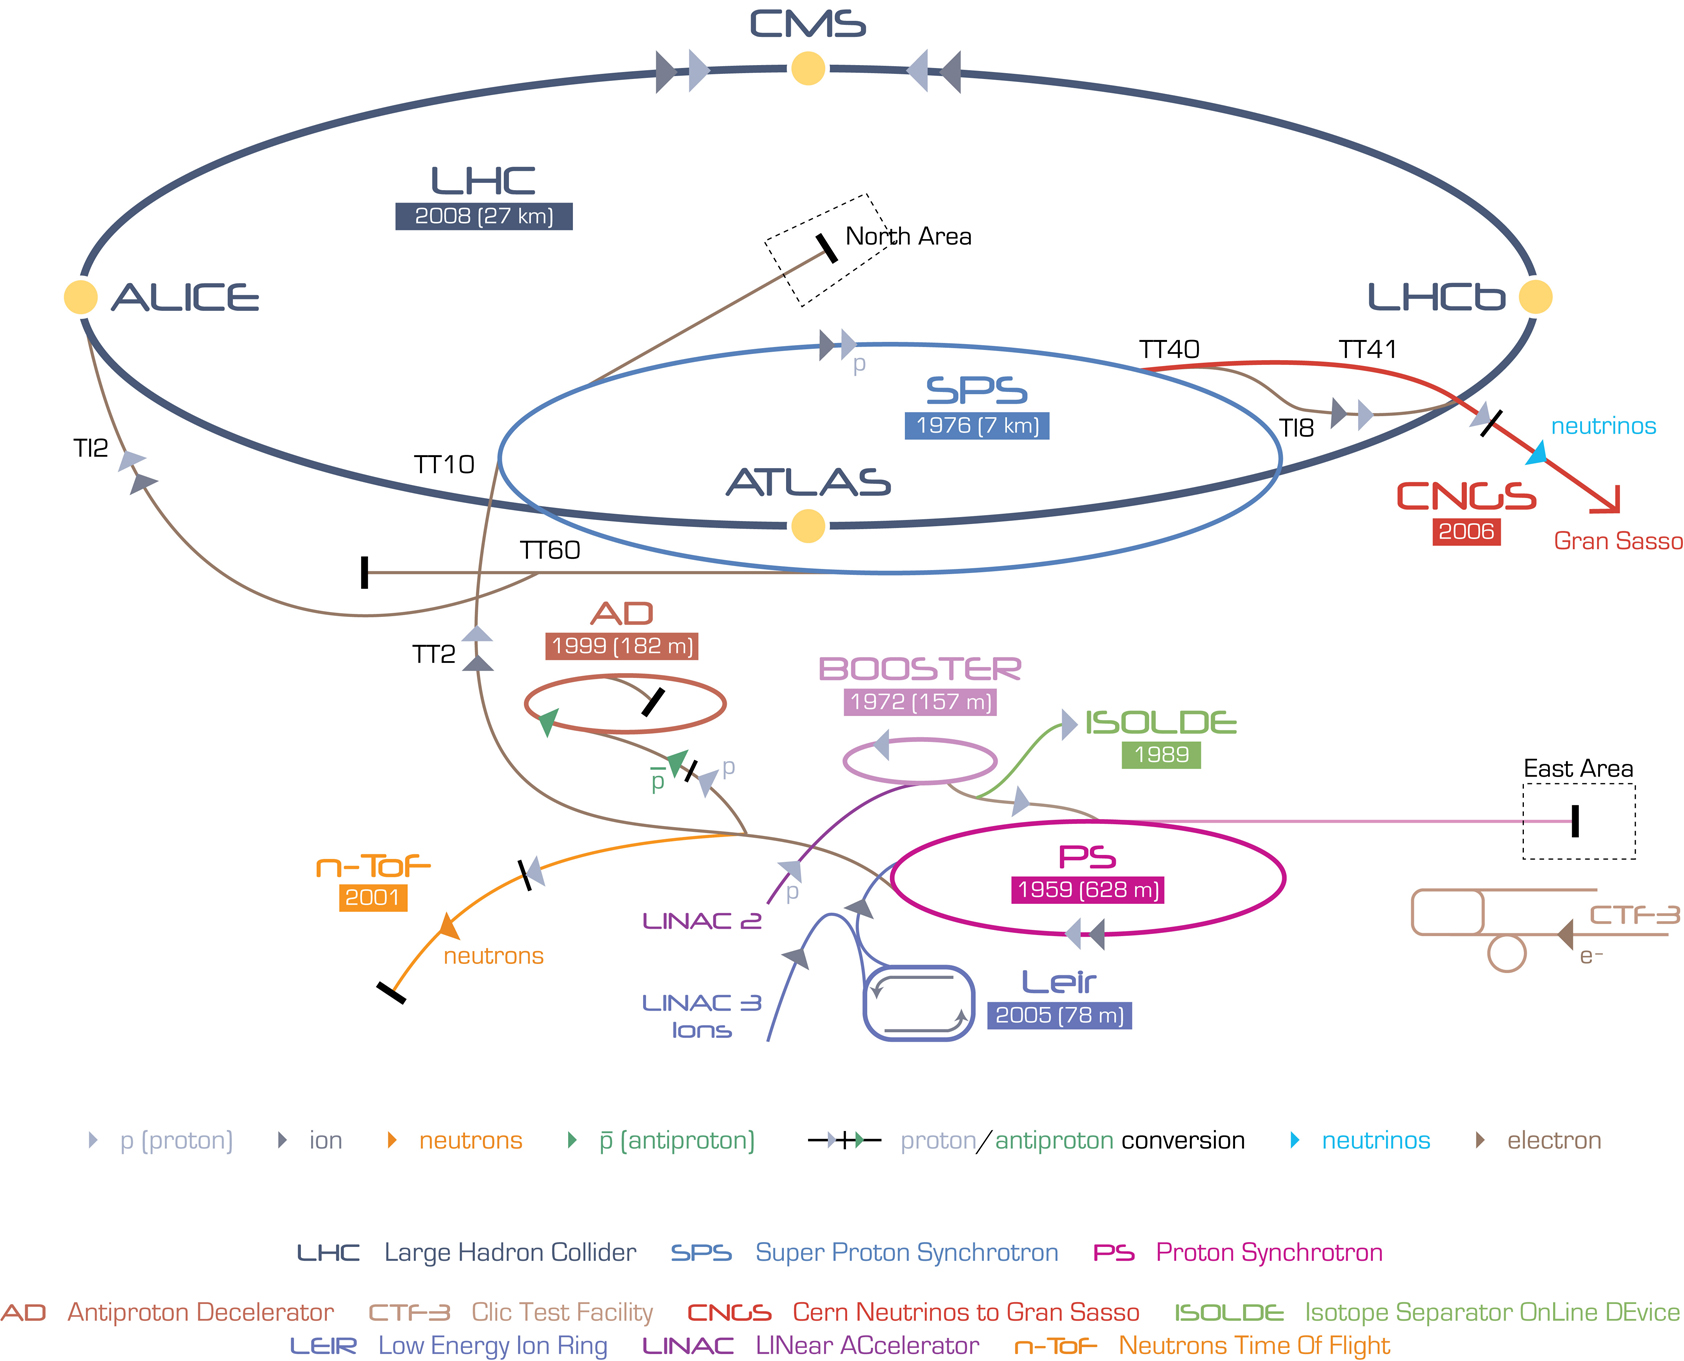
\includegraphics[width=0.95\textwidth]{PartDetector/Diagrams/Cern-Accelerator-Complex.jpg}
  \caption{The layout of CERN complex of experiments, note the main four LHC experiments located at different points around the ring.}
  \label{fig:DetectorLHCLayout}
\end{figure}

The LHC accelerates two beams of protons in opposite directions and then collides the two beams at the four interaction points where the experiments are located. The protons come from hydrogen gas where the orbiting electron is removed by an electric field, leaving behind a bare proton. The beam acceleration occurs in several stages exploiting smaller experiments present at CERN. During 2010 and 2011 protons were accelerated to a beam energy of 3.5 TeV, creating a centre-of-mass energy of 7 TeV and then 4 TeV per beam in 2012 for a centre-of-mass energy of 8 TeV. Each beam is made of multiple bunches of protons, with as many as hundreds of billions of protons in each bunch. Bunches are grouped into \textit{bunch trains} with a designed \textit{bunch spacing} of 25 ns between each of the bunches that compose a single train. Note that the bunch spacing and size of the bunch can be altered to adjust the amount of collisions and the time between collisions. The variation in the number of colliding bunches is shown in Figure~\ref{fig:DetectorBunchesColliding}.

\begin{figure}[tbhp]
  \centering
  \begin{subfigure}[b]{0.95\textwidth}
    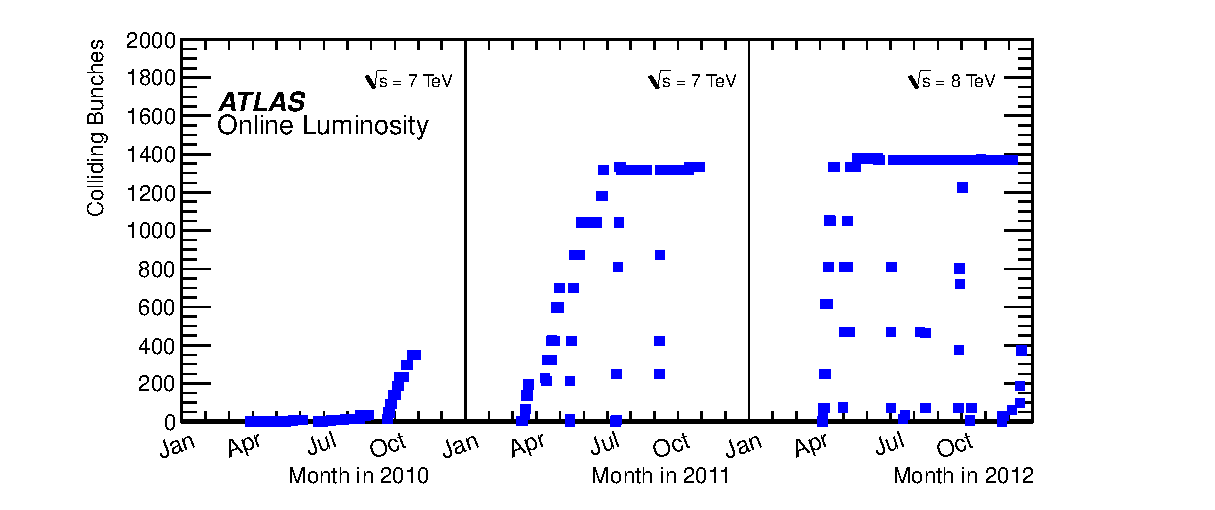
\includegraphics[width=\textwidth]{PartDetector/Plots/BunchesCollidingPerTime.eps}
    \caption{The number of bunches colliding per unit time at the LHC for the 2010, 2011 and 2012 $pp$ collision periods.} \label{fig:DetectorBunchesColliding}
  \end{subfigure}
  
  \begin{subfigure}[b]{0.95\textwidth}
    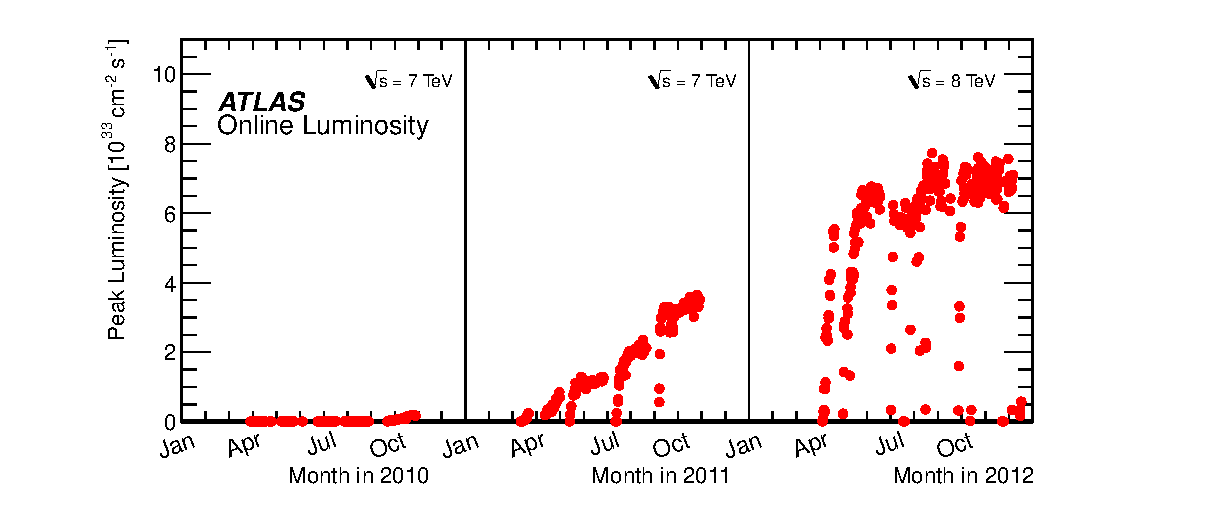
\includegraphics[width=\textwidth]{PartDetector/Plots/PeakLuminosityVsTime.eps}
    \caption{The peak luminosity per unit time at the LHC for the 2010, 2011 and 2012 $pp$ collision periods.} \label{fig:DetectorPeakLumi}
  \end{subfigure}
  \caption{Shown in \subref{fig:DetectorBunchesColliding} is the number of bunches colliding at the LHC and \subref{fig:DetectorPeakLumi} the peak luminosity per unit time.} \label{fig:DetectorPerformance}
\end{figure}

The acceleration of the proton beams occurs in several stages, within several different accelerators. The beams are first accelerated in a linear collider (LINAC 2) to an energy of 50 MeV before being injected into the proton synchotron booster (PSB). The beams are then boosted to 1.4 GeV by a varying magnetic field in the circular PSB. The beams are then passed into the proton synchrotron (PS) and then the super proton syncrotron (SPS) where the beam energy increases to 26 GeV and then 450 GeV. At this stage the beam is injected into the LHC and then accelerated to the final desired energy. The design energy is 7 TeV per beam for a total of 14 GeV centre-of-mass energy. From injection of the protons into LINAC 2 to stable beam conditions in the LHC, the whole process can take a couple of hours.

As bunches overlap the protons that make up the bunches interact, these interactions are known as events. The number of events is proportional to the instantaneous luminosity $\Lagr$ of the collider. $\Lagr$ is a measure of the flux of particles per unit area per unit time can be defined as:

\begin{equation}
  \Lagr=f{n_b}\frac{N_1 N_2}{A}
\end{equation}
%
where $f$ is the frequency of revolution of the beam, $n_b$ the number of colliding pairs of bunches in the beam, $N_1$ and $N_2$ are the number of particles in each colliding bunch and A is the cross-section of the beam~\cite{Luminosity}. The peak luminosity evolution at the LHC is shown in Figure~\ref{fig:DetectorPeakLumi}. Note that the operational $\sqrt{s}$ of the LHC was 7 TeV for 2010/11 and 8 TeV for 2012.

The total amount of data collected is measured by the integrated luminosity $\Lagr_{\textrm{int}}$ defined as the time integral of $\Lagr$. Integrated luminosity has units of inverse area, usually expressed in terms of barns (b)\footnote{1 $b^{-1}$ = $10^{-28}$ $m^{-2}$}. The probability for a given process to occur is expressed as the cross-section $\sigma$ and the total number of events which proceed via said process is defined as:
%
\begin{equation}
  \sigma\int\Lagr\,\mathrm{d}t
\end{equation}

The integrated luminosity delivered by the LHC and collected by the ATLAS detector in 2011 and 2012 is shown in Figure~\ref{fig:DetectorIntLumi}. The ATLAS detector does not record all data delivered by the LHC; approximately $6.5\%$ was not recorded.

\begin{figure}[htbp]
  \centering
  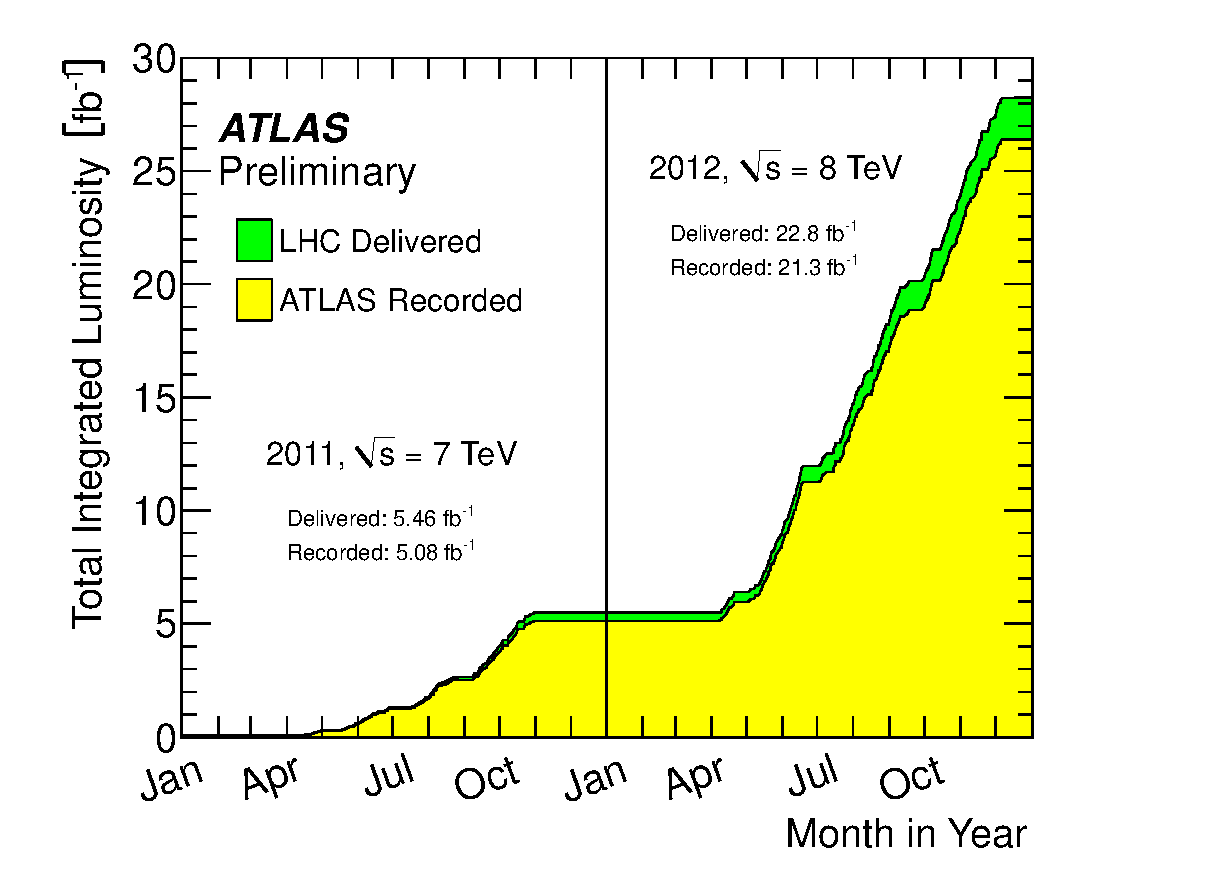
\includegraphics[width=0.65\textwidth]{PartDetector/Plots/IntegratedLuminosity20112012.eps}
  \caption{Distribution of the total integrated luminosity delivered by the LHC and the recorded by ATLAS for the 2011 and 2012 $pp$ collision period. Note the $\sqrt{s}$ changing from 7 TeV to 8 TeV between 2011 and 2012.}
  \label{fig:DetectorIntLumi}
\end{figure}

\subsection{Pileup}

Due to the large number of interactions and the short time between collisions, multiple events can overlap into a single event. This has detrminetal effects on physics analyses and is a determining factor in setting the instantenous luminosity with which to perform data collection. This overlapping effect is collectively known as pileup and is categorized into two types: in-time pileup, where multiple $pp$ collisions occur during the same bunch crossing; and out-of-time pileup, where the electric signals produced by a previous collision is still present in the detector. The number of interactions per crossing $\mu$ is shown in Figure~\ref{fig:DetectorBunchCrossingInteractions}, note that on average approximately thirty interactions occurred per bunch crossing in 2012. In comparison, in 2011 the average interactions per bunch crossing $<\mu>$ varied from $<\mu>=5$ in early 2011 to $<\mu>=15$ at the end of the year. The large number of overlapping events has a detrimental effect on physics analyses and thus is an important factor when setting the operational $\Lagr$ of the collider.

\begin{figure}[htbp]
  \centering
  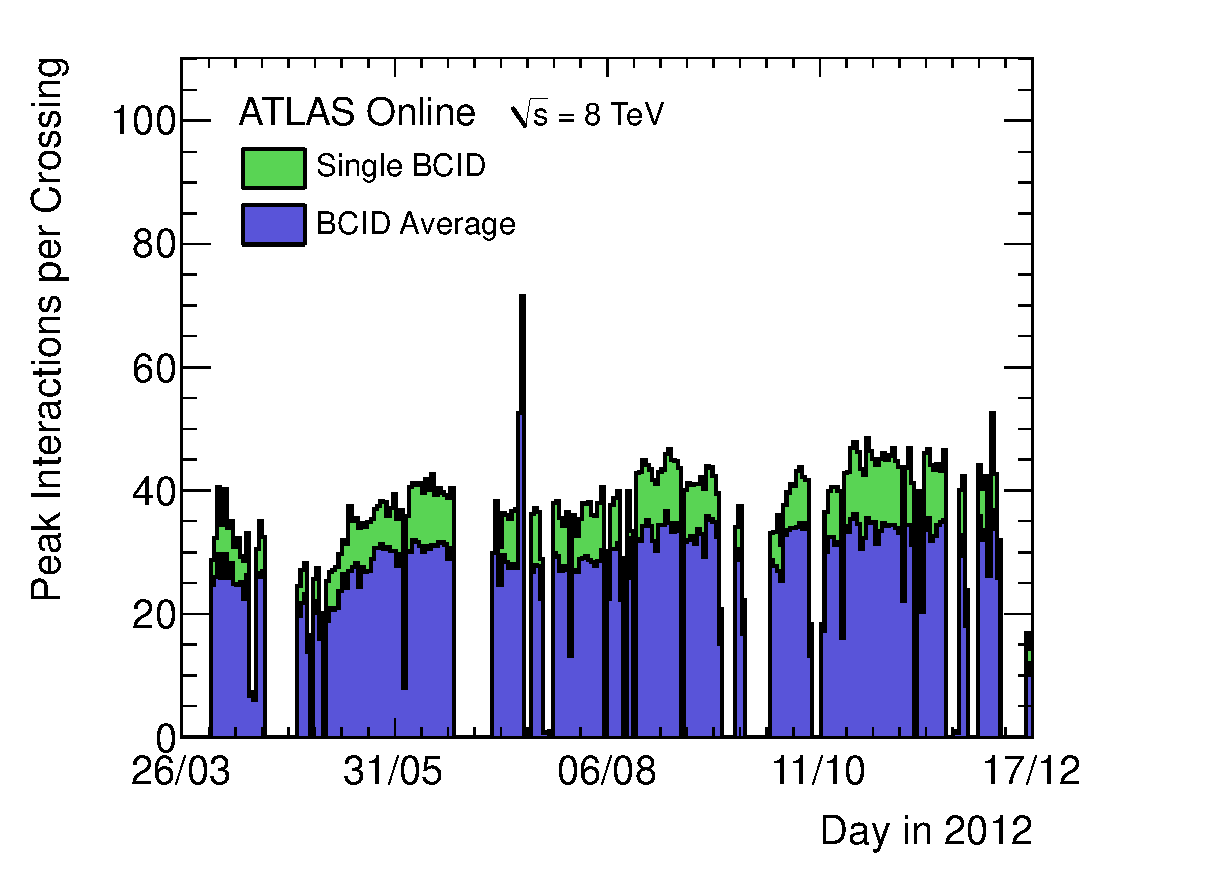
\includegraphics[width=0.65\textwidth]{PartDetector/Plots/peakBothMuByDay.eps}
  \caption{Number of interactions per bunch for the 2012 $pp$ data-taking period at ATLAS per day. Note that both the average number of interactions for all bunches and the maximum number of interactions are shown.}
  \label{fig:DetectorBunchCrossingInteractions}
\end{figure}

\section{The ATLAS detector} \label{sec:the_atlas_detector}

The ATLAS\cite{Detector:ATLASExperimentGeneral} experiment is a general-purpose detector which wraps around the IP providing large angular coverage. ATLAS is approximately cylindrical with a diameter of 25m, a total length of 44m and weighs 7000 tonnes. The detector is made of several layers of instrumentation located at succesively increasing radii as shown in Figure~\ref{fig:ATLASOverviewFigure}:

\begin{enumerate}
  \item \textbf{Inner Detector}: Located nearest to the beam-pipe and designed to measure the track of charged-particles.
  \item \textbf{EM Calorimeter}: Used for identification and measurement of electrons and photons.
  \item \textbf{Hadronic Calorimeter}: Used for the measurement of hadronic activity from hadronizing partons and missing transverse energy.
  \item \textbf{Muon Spectrometer}: The outermost detection layer, used for muon identification and measurement.
\end{enumerate}

Between these detection layers are magnets responsible for bending the path of the charged particles for the purpose of momentum measurement and particle identification. Additionally triggering and data acquisition (DAQ) systems form part of the detector for the purposes of recording the data signals coming from the aforementioned tracking and measurement systems. A brief description of these systems is provided in the coming sections. For a more detailed technical description of the detector and all subsystems see~\cite{Detector:ATLAS_TDR_vol1}.

Semi-leptonic \ttbar\ events produce a final state that includes hadronic activity, electrons, muons and missing energy and thus all elements of the detector are used in the reconstruction of such events. Additionally the match \xsm-tagger which is central to this thesis relies on the reconstruction and fitting of inner detector tracks and muon spectormeter tracks. A detailed description of this algorithm is provided in the Chapter~\ref{prt:cross_section}. 

\begin{figure}[htbp]
  \centering
  \includegraphics[width=0.85\textwidth]{PartDetector/Diagrams/ATLAS_Overall.eps}
  \caption{An overview diagram of the ATLAS experiment. Shown are all detection and tracking systems and the toroid magnet which encompasses them. Note also the muon system on the outside of the detector.}
  \label{fig:ATLASOverviewFigure}
\end{figure}

A cylindrical coordinate system as used by all ATLAS publications has been adopted here. The coordinate system is constructed so that the $z$-axis is parallel to the beam axis. The $x$-axis is positive in the direction going from the IP to the centre of the LHC ring, and the positive $y$-axis points upwards. Thus the $x-y$ plane is transverse to the beam direction. All transverse variables such as the transverse momentum \pt, transverse energy \Et\ and missing transverse energy \met\ are measured along this plane. The azimuthal angle $\phi$ is measured around the beam axis, and the polar angle $\theta$ is the angle from the beam axis. The pseudorapidity is defined as $\eta=-\ln\tan(\theta\div 2)$. The distance in the $\phi$-$\eta$ plane between two objects is denoted by $\Delta R$ and defined as $\Delta R = \sqrt{\Delta\phi^{2} + \Delta\eta^{2}}$. Finally side A of the detector is defined as the positive $z$ side and side C is the negative $z$.

\subsection{Inner Detector}
The inner detector (ID) is a tracking detector located closest to the beam-pipe and used for momentum and impact parameter measurement, vertex and track reconstruction and particle identification. The ID is designed to provide hermetic, high-resolution tracking in the range $|\eta|<2.5$. All components of the ID subsystem are shown in Figure

\begin{figure}[htbp]
  \centering
  \includegraphics[width=0.65\textwidth]{PartDetector/Diagrams/ATLAS_ID.eps}
  \caption{caption}
  \label{fig:DetectorIDOverview}
\end{figure}

The entire ID is contained within the central solenoid (CS) that generates a 2~T magnetic field for the purpose of momentum measurement. The trajectory of a charged particle is bent in the presence of a magnetic field. The str by a magnitude dependent on the momentum of the particle. By reconstructing this trajectory the momentum can be measured. 

The reconstruction of interaction vertices is of paramount importance, particularly when considering the large amount of pile-up observed at ATLAS. Interaction vertecies are reconstructed by fitting all reconstructed tracks to a point. The primary vertex (PV) is then defined as the vertex with the largest amount of momentum associated with it. In addition the reconstruction of secondary interaction vertecies is used for the identification of short-lived particles such as $B$-hadrons and $\tau$.

\begin{figure}[htbp]
  \centering
  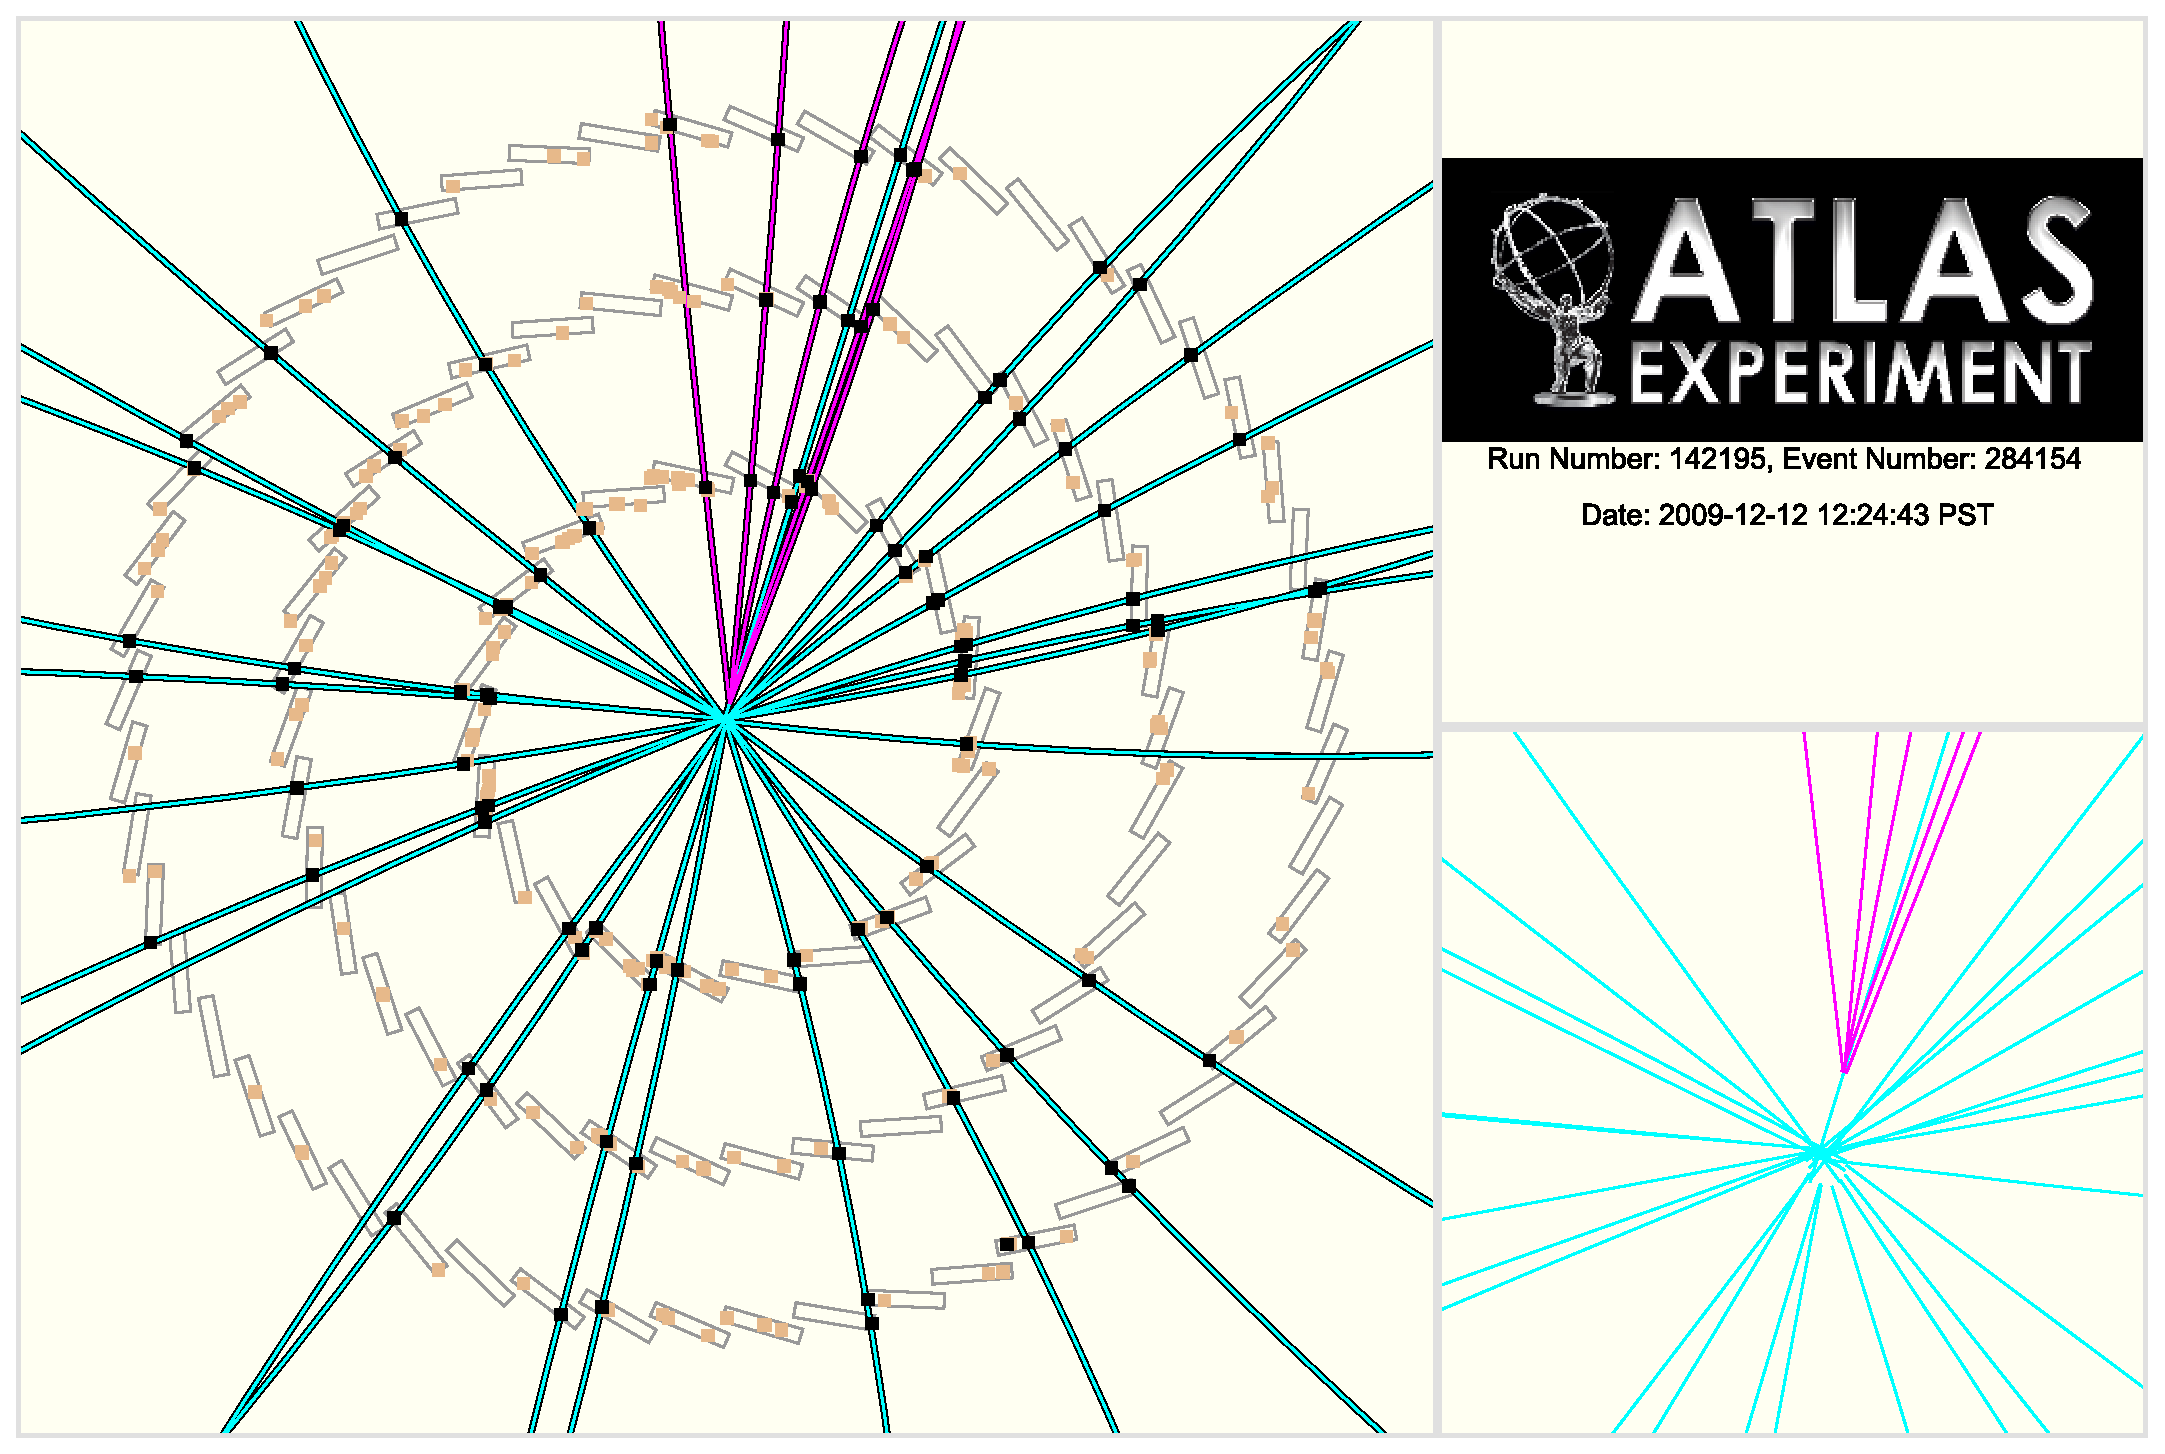
\includegraphics[width=0.95\textwidth]{PartDetector/Diagrams/fig_14.eps}
  \caption{An event-display of an event as reconstructed by the ATLAS inner detector. Shown are the results of the vertexing algorithm where each line represents a track. the purple tracks have been fitted to a secondary vertex.}
  \label{fig:label}
\end{figure}

The ID is made of three separate tracking and detection systems located at increasing radii away from the beam-pipe, the full arrangement can be seen in Figure~\ref{fig:DetectorIDQuarter} and a plane-view is shown in Figure~\ref{fig:DetectorIDTransverse}.

\begin{figure}[htbp]
  \centering
  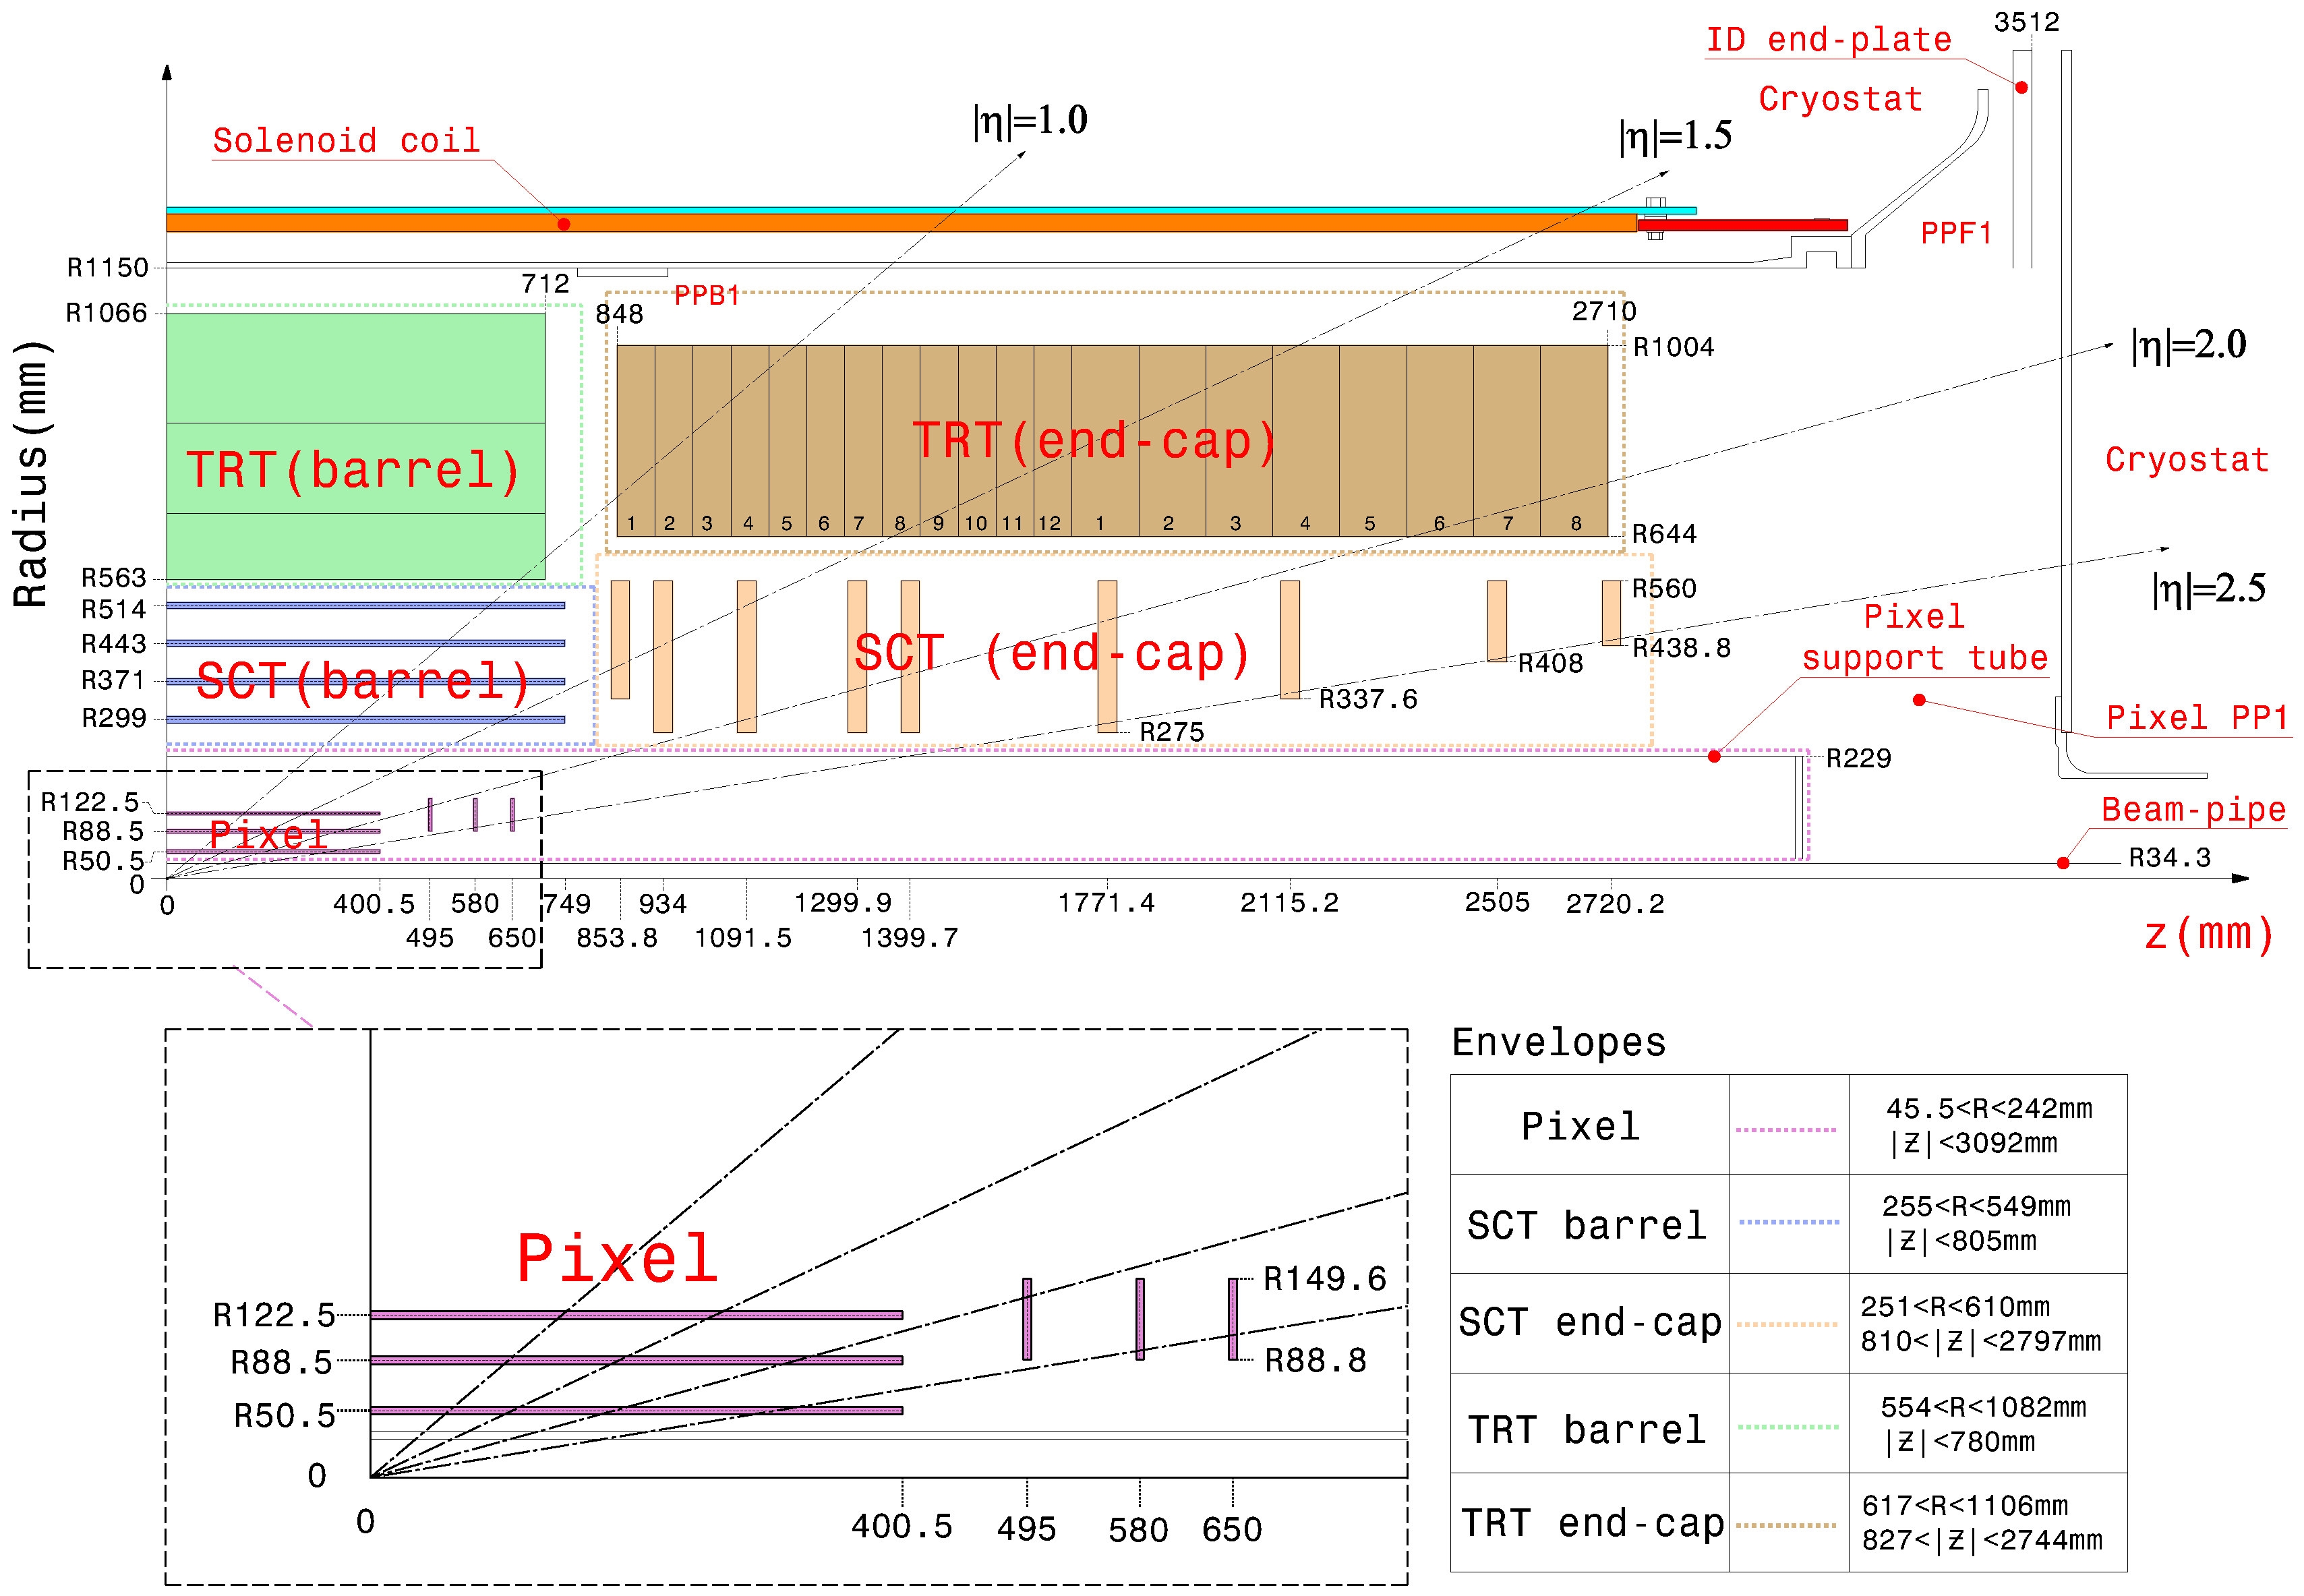
\includegraphics[width=0.75\textwidth]{PartDetector/Diagrams/Detector_ID_QuarterView.eps}
  \caption{Plan-view of a quarter-section of the ATLAS ID showing the major detector elements with its active dimenstions and envelopes. Note also the $\eta$ markers showing the maximum coverage up to $\eta=2.5$.}
  \label{fig:DetectorIDQuarter}
\end{figure}

\begin{figure}[htbp]
  \centering
  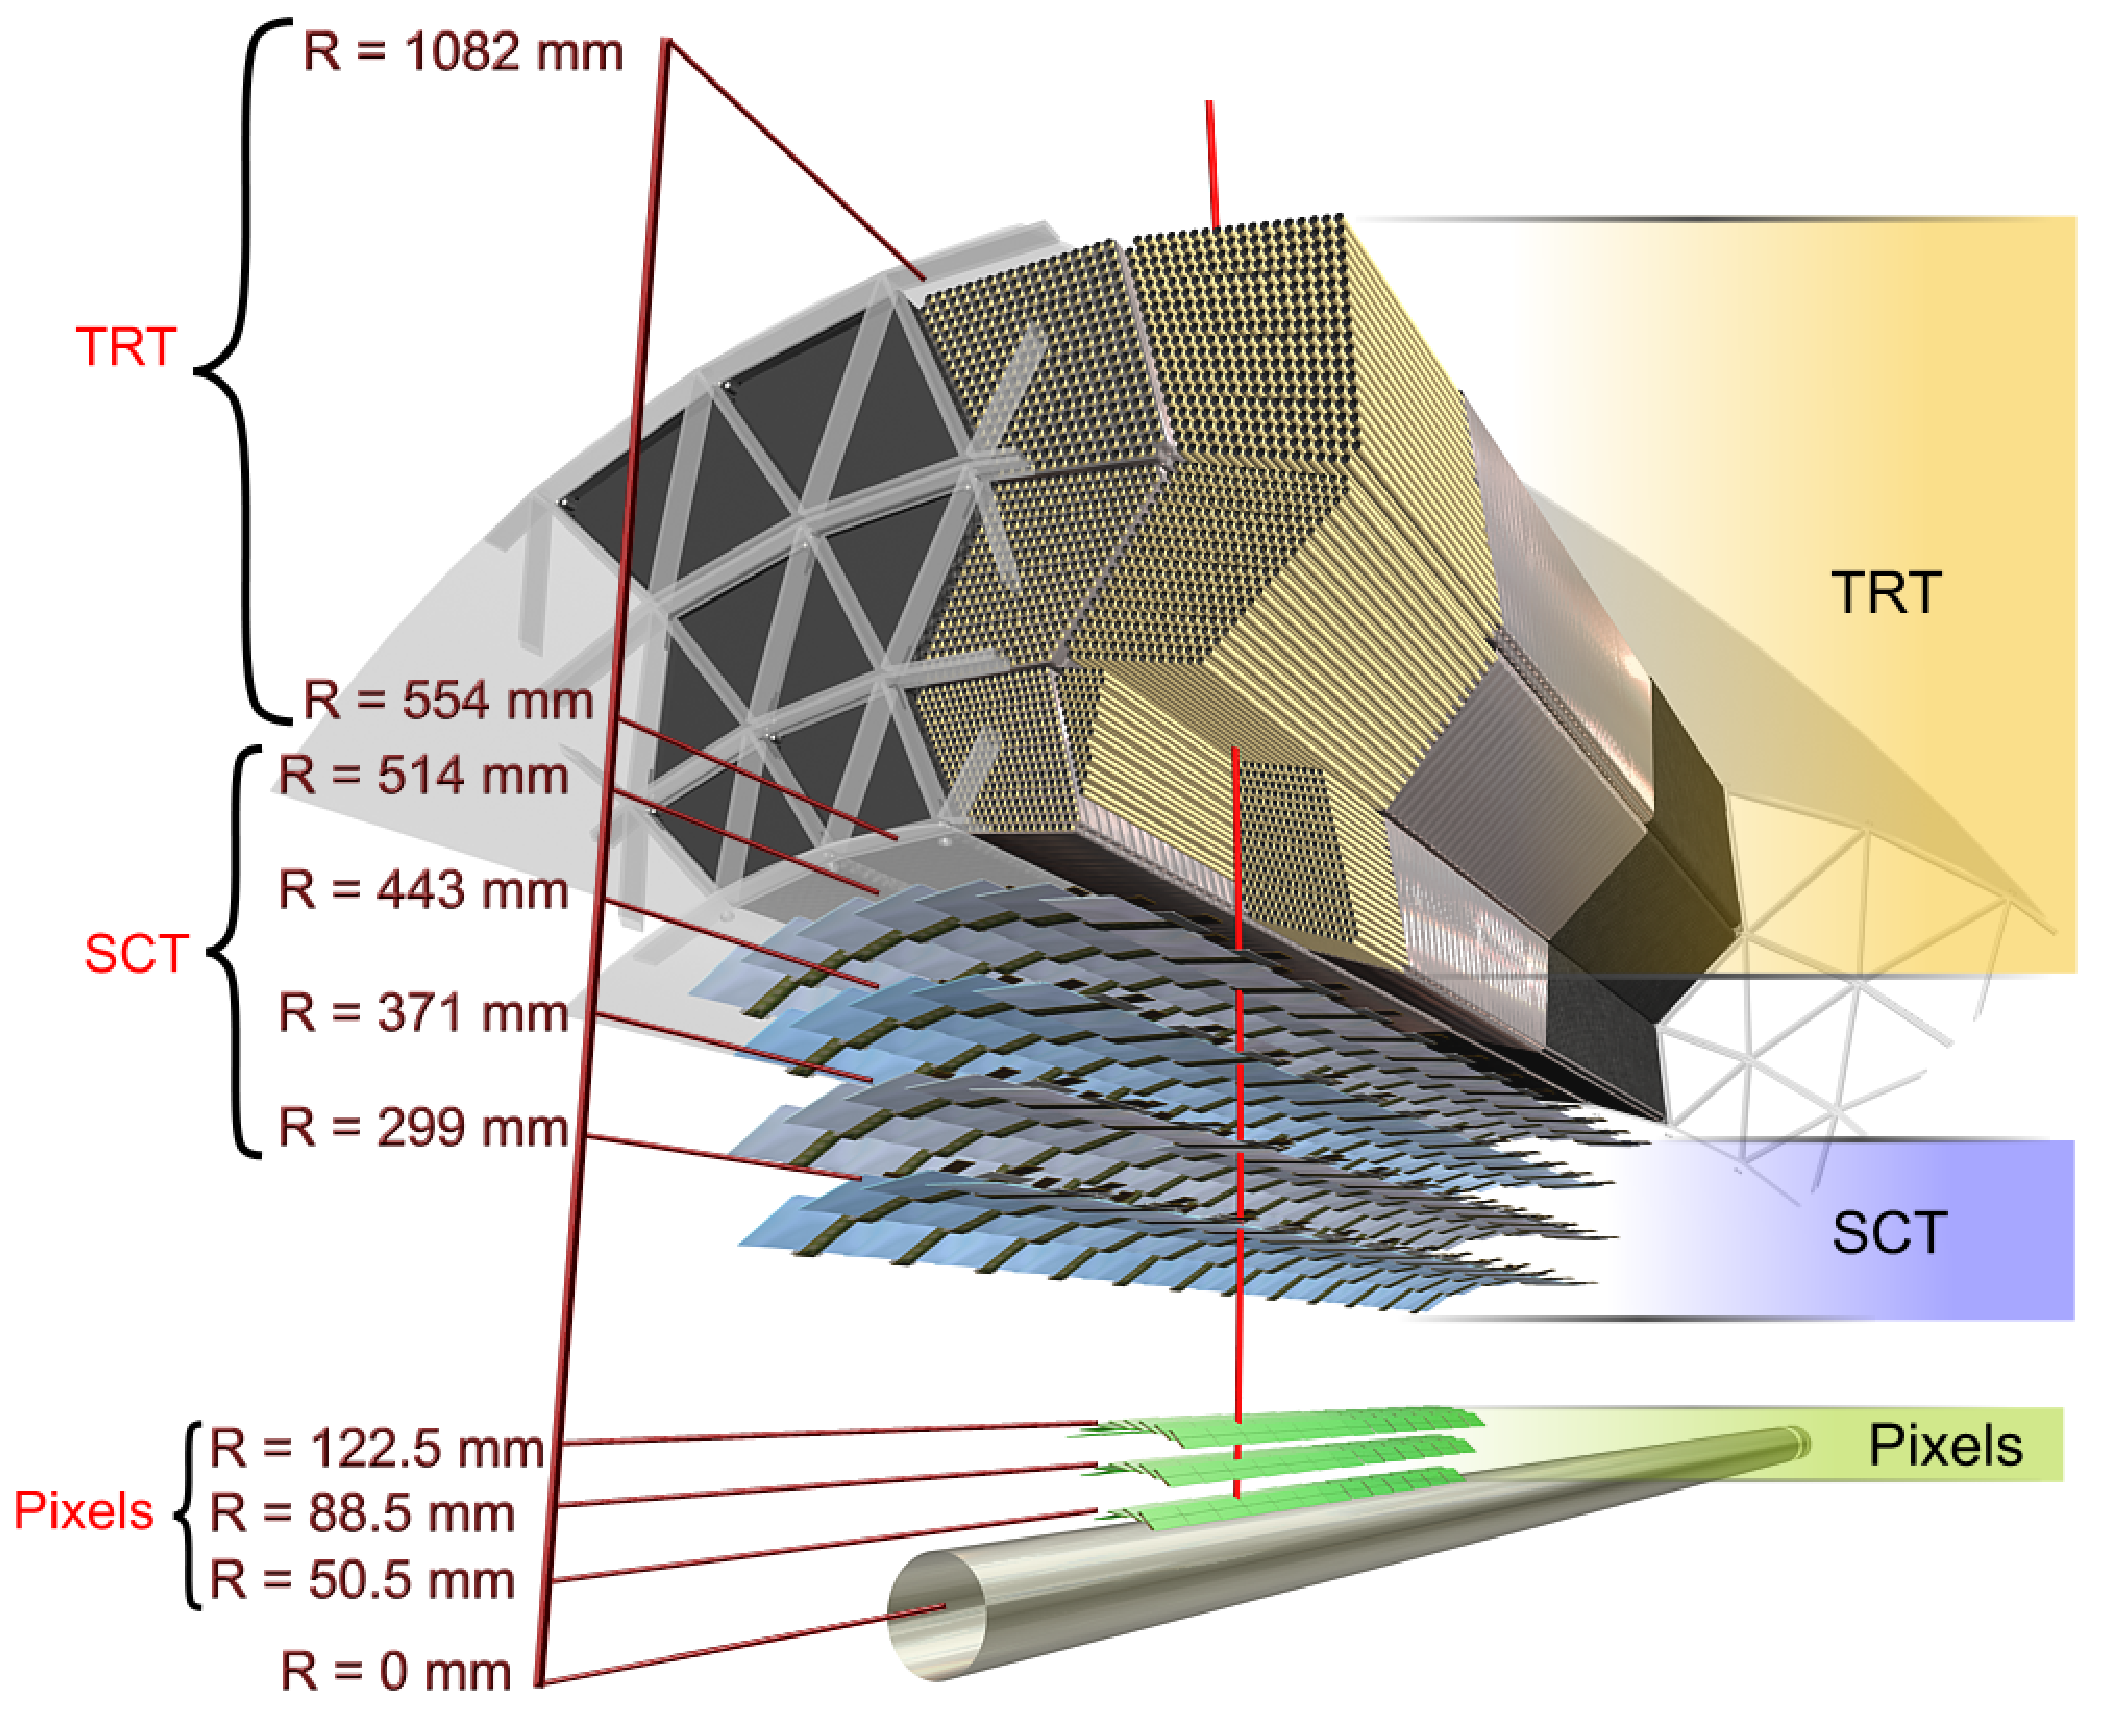
\includegraphics[width=0.75\textwidth]{PartDetector/Diagrams/ID_3D_Overview.eps}
  \caption{A drawing of in the transverse plane of the ATLAS ID showing all major detection elements in the barrel regions. Note the charged particle track marked in red traversing all the detector eleemnts.}
  \label{fig:DetectorIDTransverse}
\end{figure}

\subsubsection{Pixel detector}
The pixel detector is located nearest to the beam-pipe and provides high-granularity and precision for secondary vertex reconsruction. It consists of three silicon pixel sensors layers in the barrel region located at approximately 5cm, 9cm and 12cm from the IP, and three disks at each side located at constant $R$ providing coverage up to $|\eta|<2.5$. The barrel modules are overlapped in a turbine pattern to provide hermetic coverage. In the barrel region the modules provide an intrinsic resolution of 10\microm\ in \rphi\ and 115\microm\ in $z$. The disk sections have an intrinsic resolution of 10\microm\ (\rphi) and 115\microm\ ($R$).

\subsubsection{Semiconductor tracker}
The semiconductor tracker (SCT) located in the intermediate radius range is designed to provide eight hits per track contributing to the measurement of momentum, impact parameter and vertex position. The SCT is made of four layers of stereo-pair silicon micro-strip sensors in the barrel region at increasing radii with an intrinsic resolution of 17\microm\ (\rphi) and 580\microm\ ($z$). At the end-caps nine disks of silicon microstrip modules provide large $\eta$ coverage with a resolution of 17\microm\ (\rphi) and 580\microm\ ($R$).

\subsubsection{Transition radiation tracker}
The transition radiation tracker (TRT) is the outermost tracking layer that forms the inner detector. The TRT is designed to provide up to 36 hits per track using straw-tube sensors. In the barrel the 144cm long straw-tubes are arranged in modules which contain between 329 and 793 straws. The end-cap disks are made of radially distributed 36cm long straw-tubes. Each straw-tube provides an intrinsic resolution of 130\microm\ along its length. The combination of a large number of hits over a large radius allows for measurements in the TRT to be made with an accuracy that can complement those made by the pixel detector.

\subsection{Calorimetry}
The ATLAS calorimeter is responsible for the measurement of the energy of particles that emerge from the event. Sampling calorimeters are used for this purpose, layers of absorber material (passive) are placed in the path of the particles forcing them to interact and shower. The amount of energy lost by the incident particle depends on the type of material the particle traverses, the energy of the particle and the type. At high energies electrons lose energy predominantly via Bremsstrahlung, while photons lose energy via pair production. The characteristic length associated with this energy loss is a material characteristic known as the radiation length $X_0$.

For electrons the energy as a function of material traversed is 
%
\begin{equation}
  E=E_0e^{-x/X_0}
\end{equation}
%
where $E$ is the energy of the incident particle, $E_0$ is the original energy and $x$ is the distance traversed. As an electron traverses one $X_0$ of material, its energy is reduced by a factor of $1/e$. For photons the average number of photons traversing through a material length $x$ is reduced exponentially by a factor of $\frac{7}{9}X_0$.

The energy of the resulting shower is then measured by some sampling material (active) located behind the absorbers, this energy is proportional to the energy of the incident particle.

The type and thickness of material used is varied through the pseudorapidity range to improve energy measurement and reduce punch-through of particles into the muon systems behind. Due to the large amount of intense radiation produced during collisions, radiation hardness is also a driving factor in material choice.

The ATLAS calorimeter consists of the electromagnetic (EM) calorimeter, designed to measure photons and electrons covering the pseudorapdity region $|\eta|<3.2$; the hadronic calorimeter (HCal), designed to measure hadronic activity covering the pseudorapdity region $|\eta|<3.2$; and the forward calorimeter (FCal) which provides energy measurement capability in the very high pseudorapidity region $3.1<|\eta|<4.9$. As can be seen in Figure~\ref{fig:ATLASCalorimetryOverall} the calorimetry envelopes the ID and CS providing hermetic coverage symmetric in $\phi$. This is particularly important for the measurement of \met\ resulting from weakly interacting particles escaping the detector.

\begin{figure}[htbp]
  \centering
  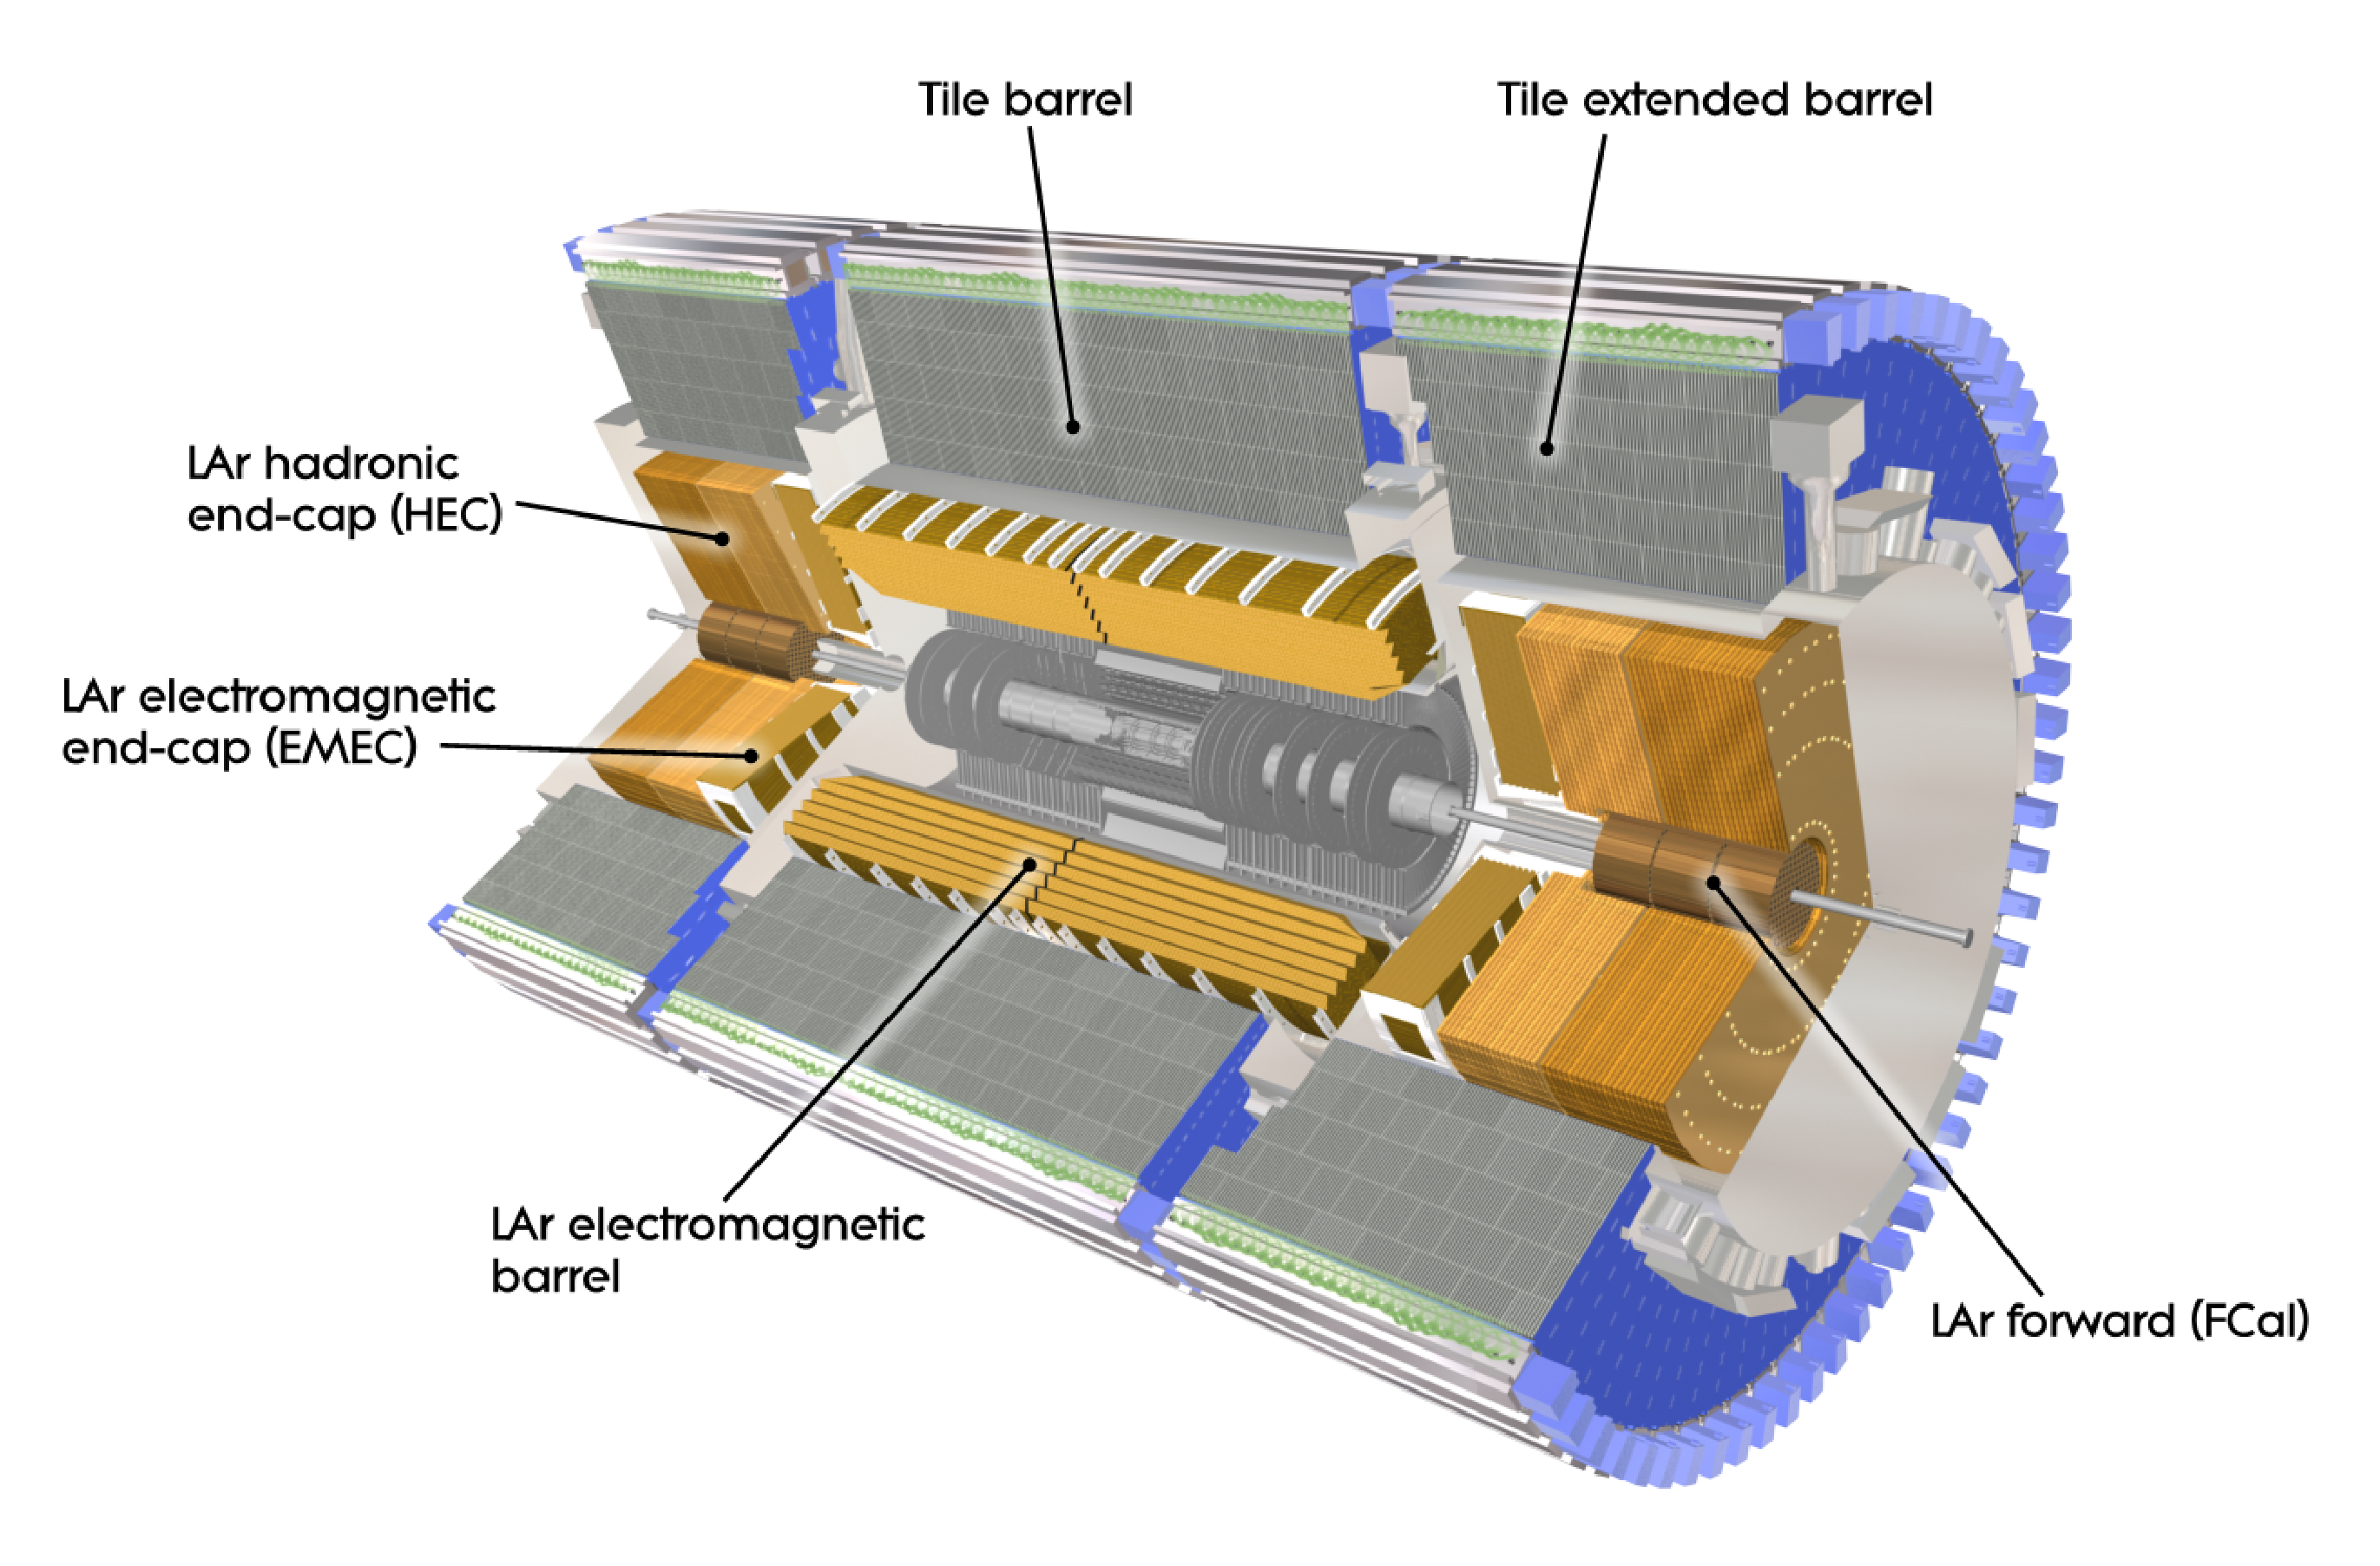
\includegraphics[width=0.75\textwidth]{PartDetector/Diagrams/ATLAS_Calorimetry.eps}
  \caption{A cut-away diagram of the ATLAS detector highlighting the calorimetry system. Shown are the ECal barrel and end-cap, the HCal barrel and end-cap and the FCal end-cap.}
  \label{fig:ATLASCalorimetryOverall}
\end{figure}

\subsubsection{Electromagnetic calorimeter}
The EM calorimeter is made of a barrel section ($|\eta|<1.475$) and two end-caps ($1.375<|\eta|<3.2$). The EM barrel consists of two half-barrels separated by a 4mm gap at $z=0$. The end-caps consist of two coaxial wheels, the outer ring covering the pseudorapidity range $1.375<|\eta|<2.5$ and the inner ring covering the range $2.5<|\eta|<3.2$. The pseudorapidity region $1.37<|\eta|<1.52$ is not used for precision physics due to the large amount of material, this is known as the ``crack'' region.

The EM calorimeter employs liquid Argon (LAr) as the active material due to its intrinsic radiation hardness and response over time, and lead as the passive material arranged in an accordion geometry for full $\phi$ symmetry. Particles interact with the lead absorbers creating a shower which ionizes the layers of liquid Argon. A potential is applied across the LAr material allowing for signal readout via Kapton/copper electrodes. The total thickness of the EM calorimeter is~$>24X_{0}$ in the barrel and $>26X_{0}$ in the end-caps. The amount of material is optimized in pseudorapidity to enhance energy resolution.

In the region devoted to precision physics the EM calorimeter is divided into three segments as shown in Figure~\ref{fig:DetectorECalSegment}, the strip layer is designed to improve particle identification and pseudorapidity position measurement. The design energy resolution for all components of the calorimeter are shown in Table~\ref{tab:DetectorCaloResolution}.

\begin{table}
  \centering
  \caption{Design energy resolution of all ATLAS calorimeter components. The resolution is made of a sampling term ($\nicefrac{1}{\sqrt{E}}$) associated with the choice of passive and active materials and construction of the layers and a constant term associated with the depth of the detector, cracks and dead material.} \label{tab:DetectorCaloResolution}
  \begin{tabular}{|l|c|}
    \hline
    Section & Resolution \\
    \hline \hline
    EM Barrel & $\frac{10\%}{\sqrt{E}}\oplus0.7\%$ \\
    EMEC & $\frac{10\%}{\sqrt{E}}\oplus0.7\%$ \\
    HEC & $\frac{100\%}{\sqrt{E}}\oplus10\%$ \\
    FCAL & $\frac{100\%}{\sqrt{E}}\oplus10\%$ \\
    \hline
  \end{tabular}
\end{table}

\begin{figure}[htbp]
   \centering
   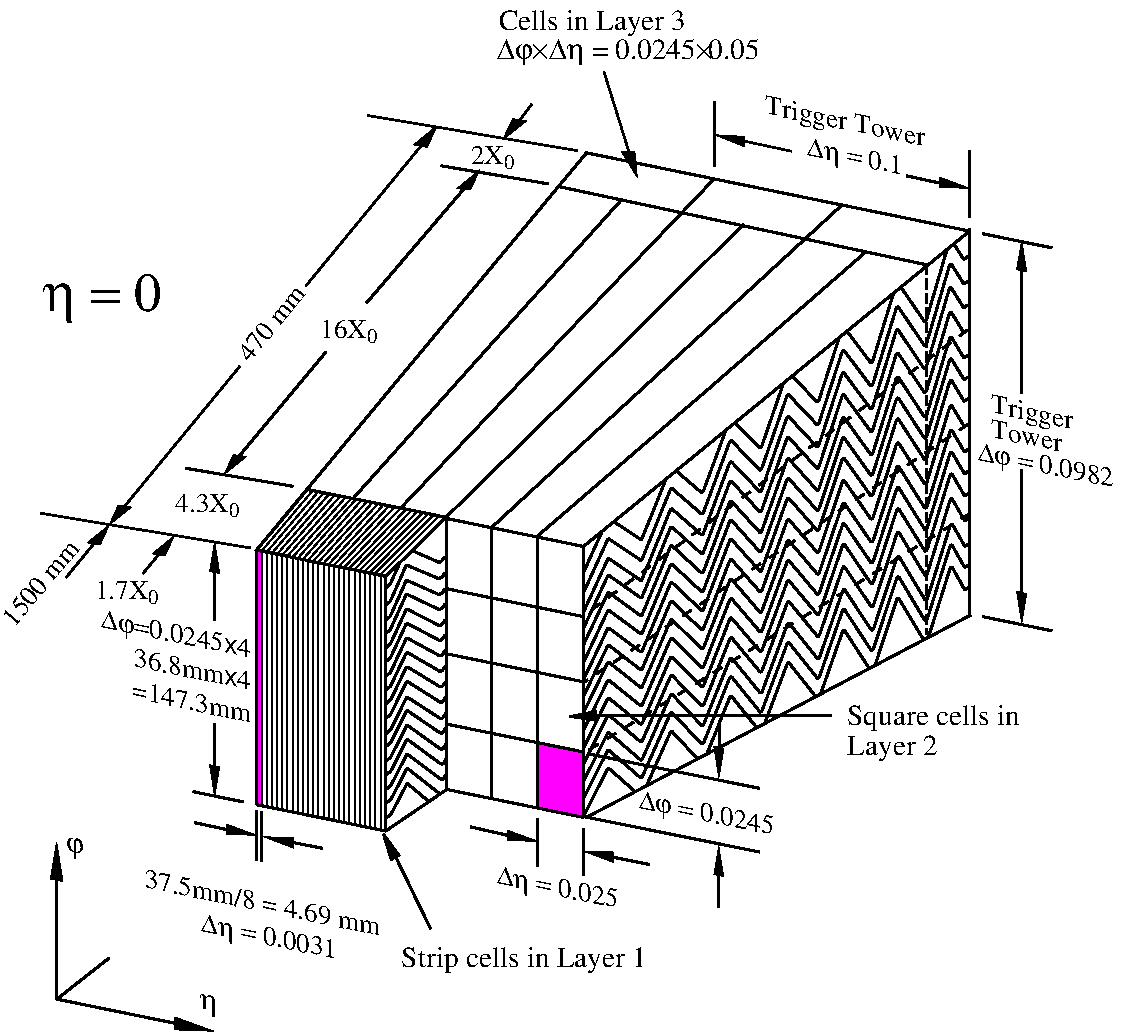
\includegraphics[width=0.75\textwidth]{PartDetector/Diagrams/LARG3-TDR-barrelM.pdf}
   \caption{Cut-away diagram of the EM calorimeter barrel at $\eta=0$. Shown are the three different layers with varying cell structures. The strip section is designed to enhance particle identification and position measurement in $\eta$.}
   \label{fig:DetectorECalSegment}
 \end{figure} 

\subsubsection{Hadronic calorimeter}
The hadronic calorimeter uses different types of passive and active material to accomodate for the varying conditions in different regions of the detector. The materials used and structure of the detector must provide good energy resolution, full symmetric coverage for the purpose of \met\ measurement,  full containment of all hardonic activity to prevent punch-through to the muon system and be sufficiently radiation hard.

The hadronic calorimeter consists of two parts a scintilator tile calorimeter in the barrel region, and a LAr calorimeter in the end-cap.

The tile calorimeter is located directly outside the EM calorimeter. The barrel portion of the calorimeter covers the region $|\eta|<1.0$ and the two extended barrels cover the range $0.8<|\eta|<1.7$. The tile calorimeter uses steel as the passive material and scintillating tiles as the active material. The resultingh hadronic showers enter the scintillating tiles and produce photons which are passed to photomultiplier tubes (PMTs). The total detector thickness which is tile-instrumented is 9.7 interaction lengths ($\lambda$) at $\eta=0$.

The hadronic end-cap (HEC) uses LAr technology due to its radiation-hardness in this challening high pseudorapidity region. The HEC consists of two independent wheels per end-cap covering the range $1.5<\eta<3.2$ overlapping the tile calorimeter at low pseudorapidity range and the forward calorimeter located at high pseudorapidity.

\subsubsection{Forward calorimeter}

The forward calorimeter (FCal) is responsible for energy measurement in the very-high pseudorapidity range $3.1>|\eta|>4.9$ of both electromagnetic and hadronic activity. Due to the large amount of radiation in this $\eta$ region, LAr is employed as the active material. The FCal consists of three layers, the first made primarily of copper, designed mostly for the measurement of electromagnetic activity while the two outer tungsten layers are responsible for hadronic activity measurement.

\subsection{Muon system}

The muon system is the outer most layer of the ATLAS detector and is responsible for the measurement of $p_{T}$ charged-particles that traverse the ATLAS calorimetry. 

\begin{figure}[htbp]
  \centering  
  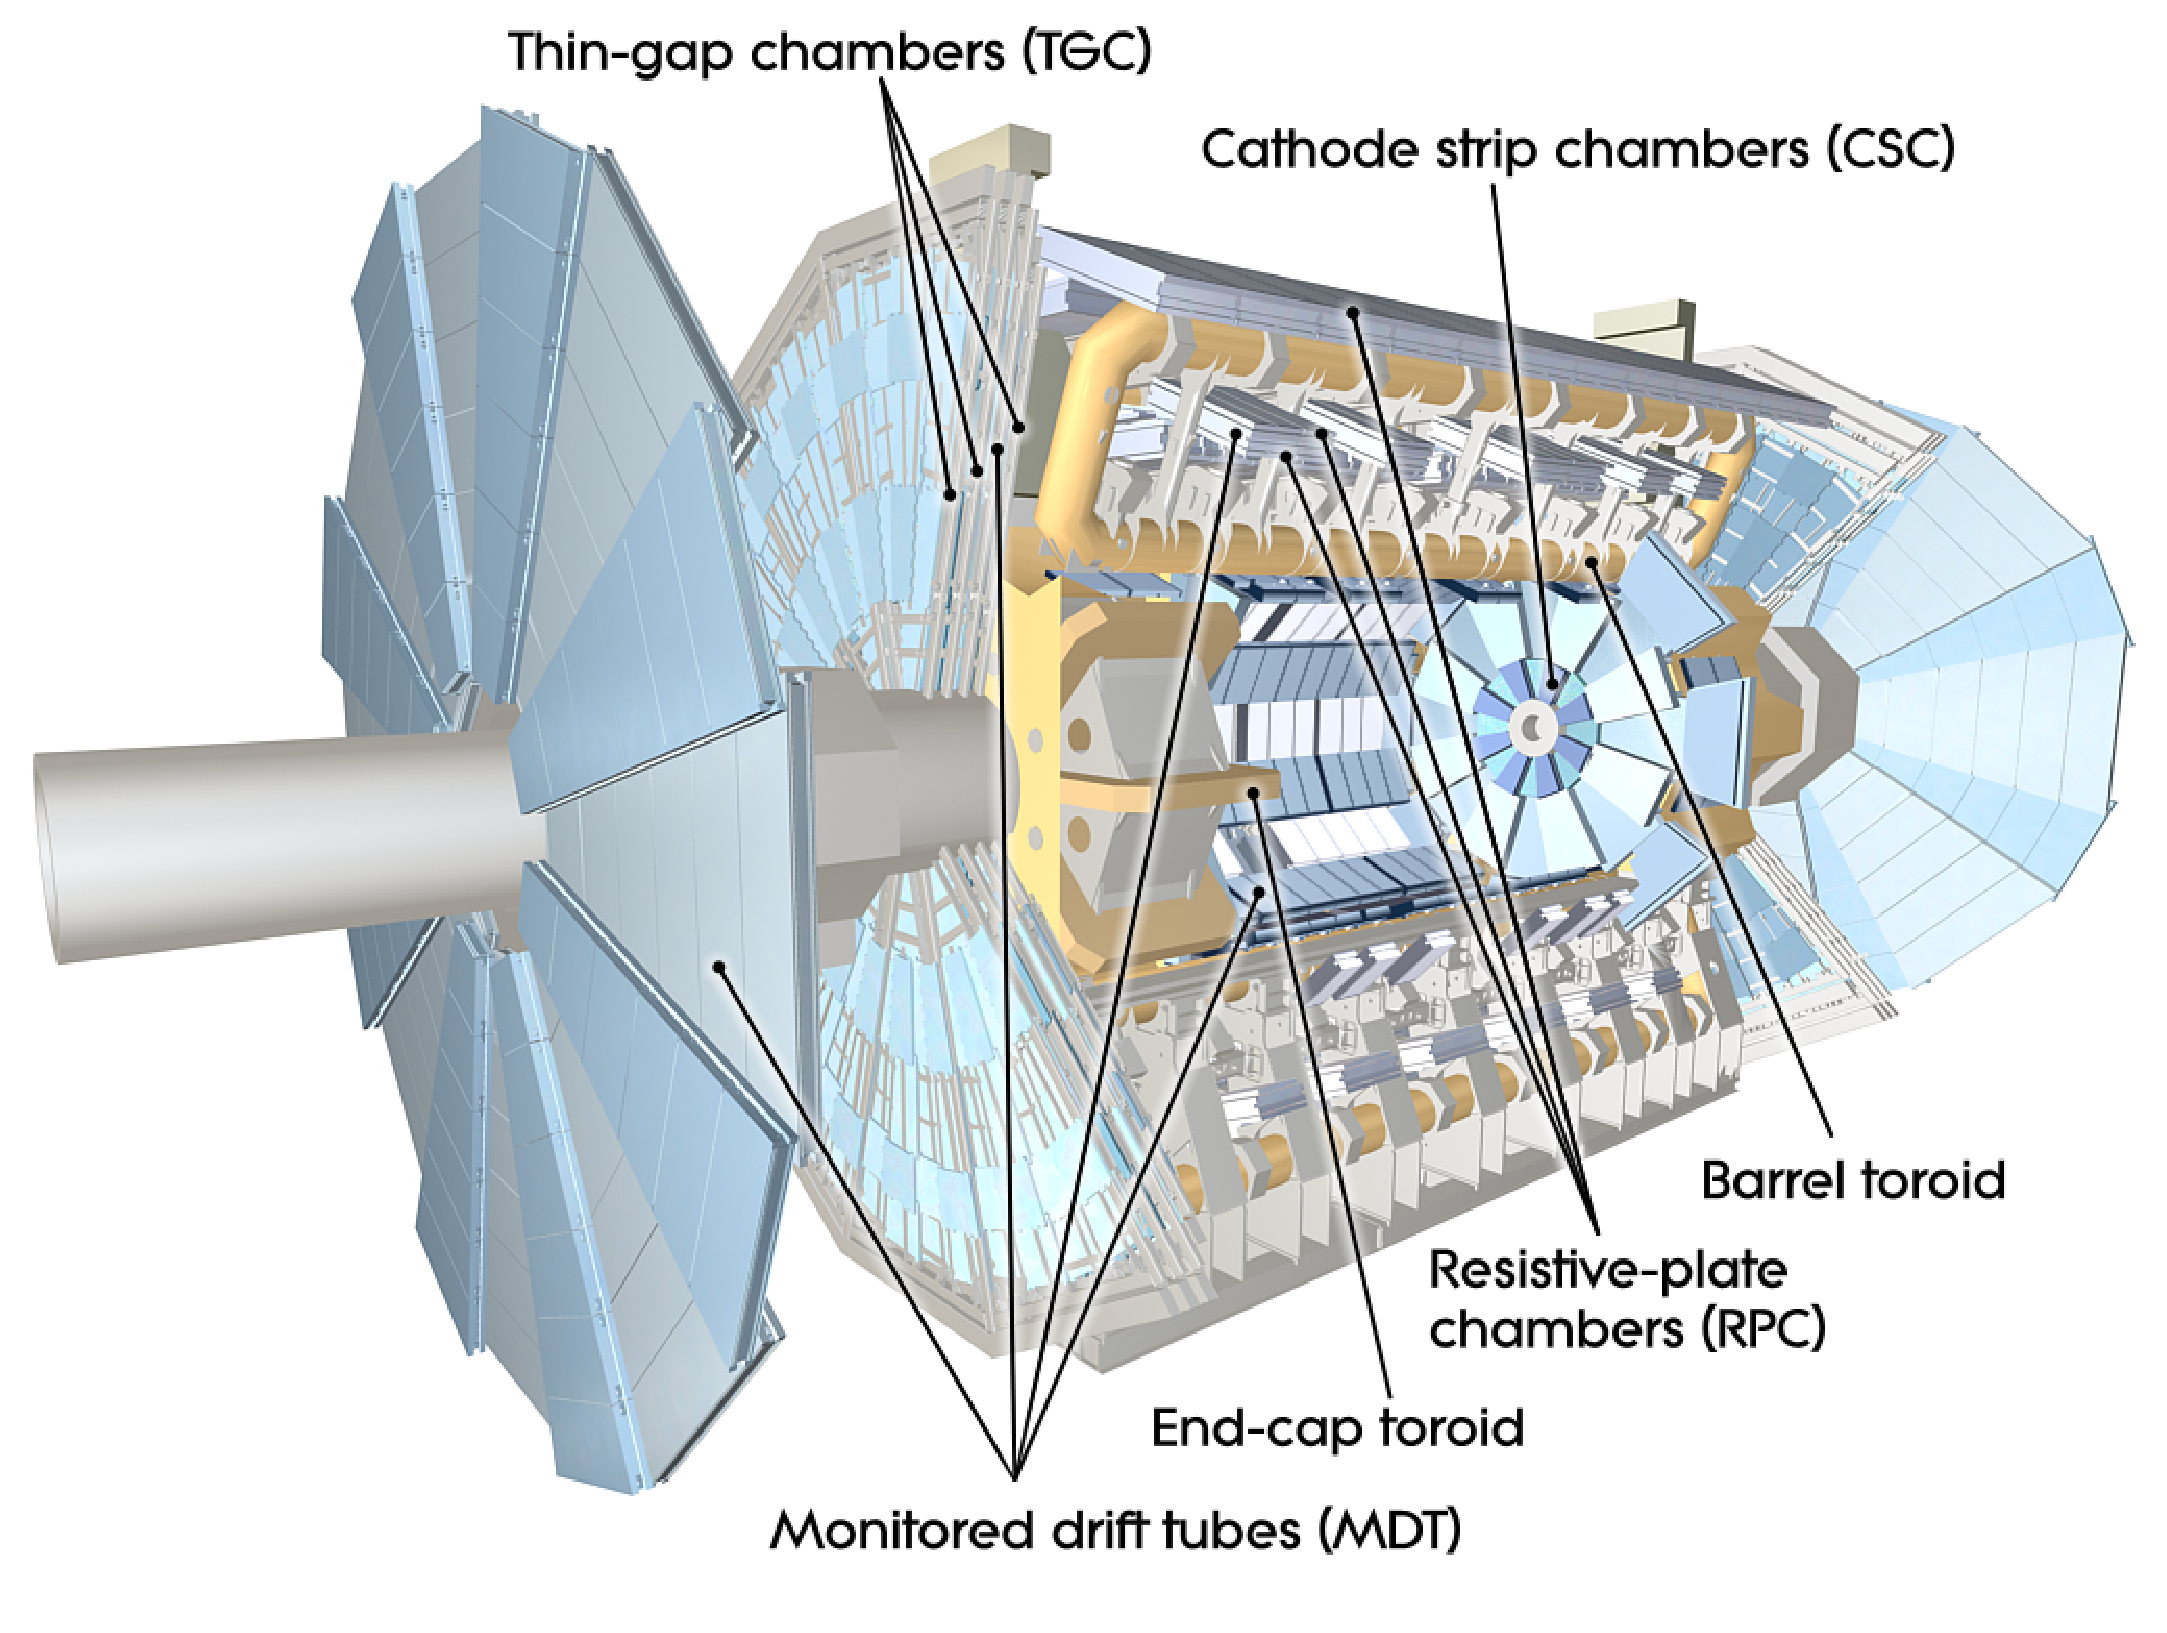
\includegraphics[width=0.95\textwidth]{PartDetector/Diagrams/ATLAS_MuonSystem.eps}
  \caption{Cut-away drawing of the ATLAS muon system.}
  \label{fig:DetectorDrawingMuonSystem}
\end{figure}

\begin{figure}[htbp]
  \centering
  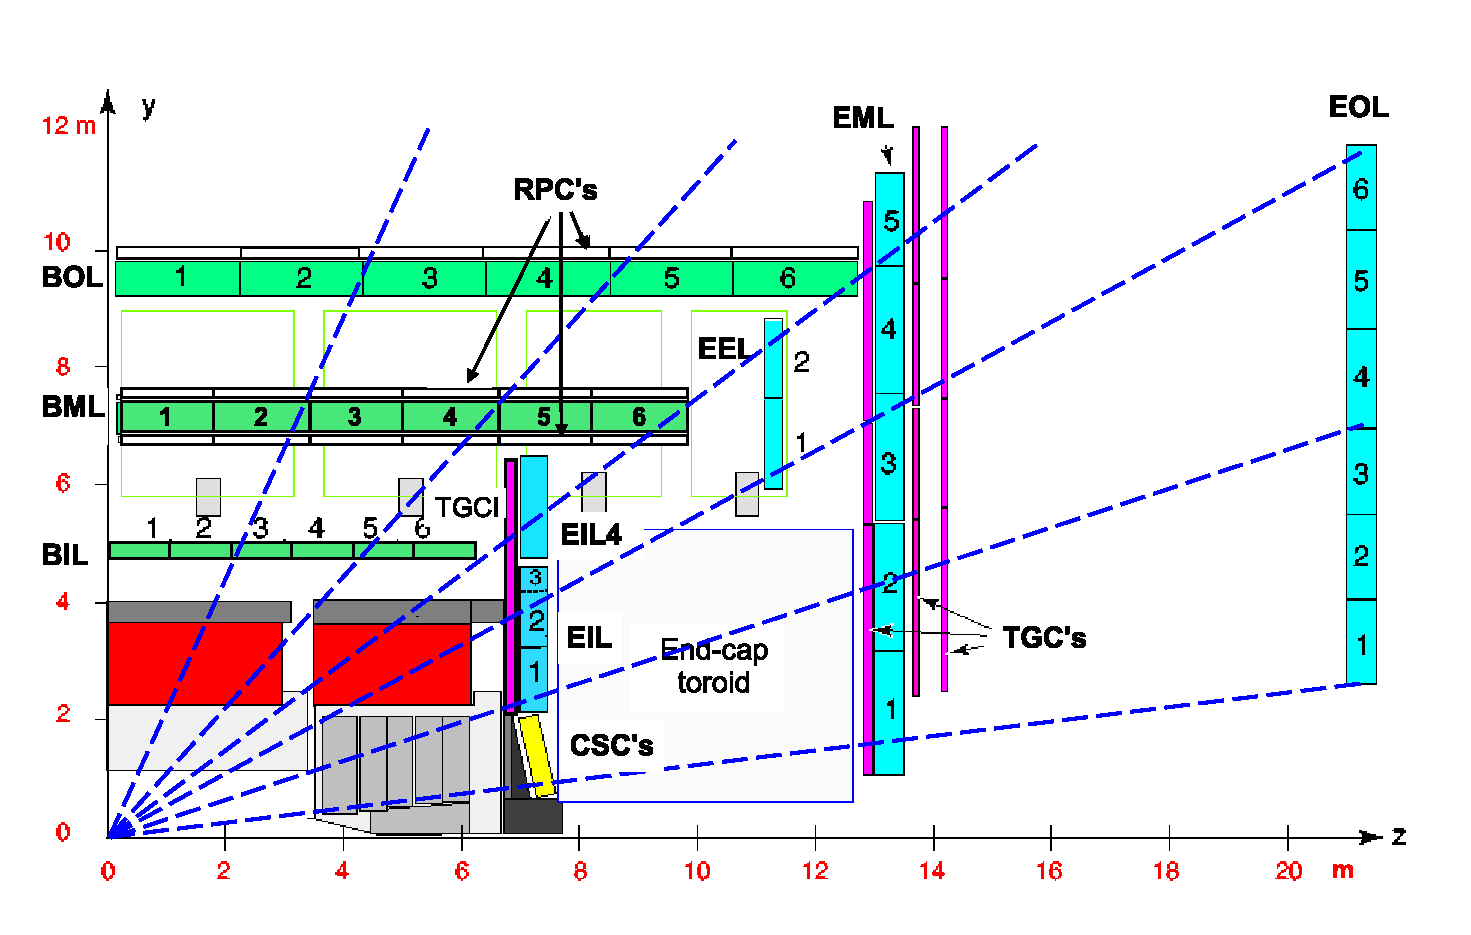
\includegraphics[width=0.95\textwidth]{PartDetector/Diagrams/Muon_section.eps}
  \caption{Plan view of quarter-section of the ATLAS muon system.}
  \label{fig:DetectorMuonOverview}
\end{figure}
\subsection{Triggering and DAQ}

\section{Athena Control Framework and ROOT Framework}
